\documentclass[]{article}
\RequirePackage{amsmath}

\usepackage{graphicx}
%\graphicspath{{./figures/}}
\usepackage{amssymb}
\usepackage{color}
\usepackage{hyperref}
\usepackage{algorithm}
\usepackage{algpseudocode}
\bibliographystyle{IEEEtran}
\newcommand{\knote}[1]{\textcolor{green}{A: {#1}}}
\newcommand{\dnote}[1]{\textcolor{red}{D: {#1}}}
\newcommand{\vk}[1]{\textcolor{blue}{V: {#1}}}
\newcommand{\lnote}[1]{\textcolor{cyan}{L: {#1}}}


\begin{document}
    \title{The Ergo Platform}

    \date{\today}
    \maketitle

    \begin{abstract}
        This document contains a general idea of Ergo platform and a high-level overview of it's main features.
        More details may be found in separate papers cited along this one.
    \end{abstract}

    \section{Vision}

    Ergo platform was started in 2017 after several years of research and prototypes implementations.
    Despite of huge hype around cryptocurrencies, the technology itself stuck close to it's initial stage.
    In pursuit of high profits and popularity, developers claimed an implementation of blockchain 2.0 (3.0 and so on),
    in prejudice of the main advantage of cryptocurrencies -- decentralization -- and promising that it will be achieved
    somewhere in the future.

    In opposite, the idea of Ergo is implement ready-to-use ideas keeping the network really decentralized.
    It may be called a blockchain 1.1 - a major update to the blockchain technology instead of
    a revolutionary breaking changes.
    The main focus of Ergo is to be the platform that is really useful for blockchain-demanded
    decentralized applications, and to be survivable in a long distance.
    Technical and economic solutions that will allow to achieve this will be described in the following sections.

    \section{Consensus}

    Consensus protocol of Ergo -- Autolykos -- is based on the well-known Proof-of-Work idea.
    PoW was chosen by several reasons: these protocols are widely studied, have high security guarantees
    and are friendly for light clients.
    However, existing PoW protocols have known drawbacks: ASIC-equipped miners produce blocks
    orders of magnitude faster than regular miners, moreover
    they unite in mining pool and just few pool operators controls the network as a result.

    The general way to reduce the advantage of ASICs is to use memory-hard computations.
    Autolykos is based on k-sum problem, that is similar to a known memory-hard Equihash PoW~\cite{biryukov2017equihash}.
    In addition, Autolykos is a variant of a Schnorr signature and thus mining is not possible without the access to private key.

    These two properties prevents the centralization of the
    network around pool operators and ASIC manufacturers, and returns Ergo back to the original
    one-CPU-one-vote idea from the Bitcoin whitepaper~\cite{nakamoto2008bitcoin}.

    \section{Clients}

    It is almost impossible to use existing cryptocurrencies without a help of trusted parties.
    To receive few coins, a client should download and process gigabytes of
    data to synchronize the network, which may take several weeks even on a high-end hardware,
    not to mention a mobile phones.
    No wonder that most of users prefer to use trusted solutions for wallets, exchanges, block
    explorers and so on.

    Ergo was designed to be maximally user-friendly in the sense of decentralization.
    One of important properties of PoW is that it allows to verify the work done without
    downloading the full chain.
    Ergo block headers supports NiPoPoW~\cite{kiayias2017non} proofs, allowing light clients
    to synchronize the network by downloading less then a megabyte of data.
%    This allows to check, that client is on the best chain, while does not allow
%    him to validate arbitrary transactions.
    In addition, Ergo use authenticated state~\cite{reyzin2017improving} and for any transaction
    included, a client may download a proof of it's correctness.
    Thus, regardless of the blockchain size, a regular user with a smartphone can
    join the network and start using Ergo with the security guaranties of the full node.

    \section{Survivability}

    Long-term survivability is important because of ...

    To survive in a long-term, Ergo prefers well-tested solutions.
    If there is no appropriate solution for some problem, we perform our own research and
    the number of peer-reviewed papers from the Ergo team is already quite big:
    ~\cite{reyzin2017improving,meshkov2017short,chepurnoy2018systematic,chepurnoy2018self,chepurnoy2018checking,duong2018multi}.

%    A key aspect of decentralization is the lack of dependence on developers.
%    This requires that at any point of time it should be able to survive without trusted parties.
    To be survivable, the network should adopt to changing environment without intervention of trusted
    parties (like a "core developers" team).
    Ergo voting protocol allows to change a lot of parameters (blocks size, contracts costs and more) via miners voting.
%    that should reduce probability of hard forks and chain splits.
    For more fundamental changes Ergo is going to follow soft-forkability approach -
    if an overwhelming majority of the network accepts a new feature, it is activated,
    however old nodes continue to operate normally just skipping this feature validation.

    \section{Economy}

    To achieve survivability, Ergo provides economic improvements in addition to the technical ones.
    Demurrage component plays important role for Ergo stability:
    once per 4 years users are enforced to pay a small fee for every byte, kept in the state, and
    if an output value is less than a required fee to pay, this output will be removed from the state.

    Thus, demurrage component is similar to regular cloud storage services, however it is new for cryptocurrencies
    and has several important consequences.
    First, Ergo mining will always be stable, unlike Bitcoin and other PoW currencies, in which
    mining may become unstable after the initial emission~\cite{carlsten2016instability}.
    Second, state size become controllable and predictable, reducing hardware requirements
    for Ergo miners.
    Third, by collecting storage fee from outdated boxes, miners return coins to circulation,
    preventing steady decrease of circulating supply due to lost keys~\cite{wsj2018}.

    Finally, it allows to stop emission quite soon.
    Ergo emission will last for 8 years - for the first 2 years 75 Erg will be issued per block
    and after that block reward will be reduced for 3 coins every 3 month~(see Fig.~\ref{fig:emission}).
    To fund the Ergo development, during the first 2.5 years part of the block reward, that
    exceeds 67.5 will go to a treasury instead of a miner.

    \begin{figure}[h]
        \centering
        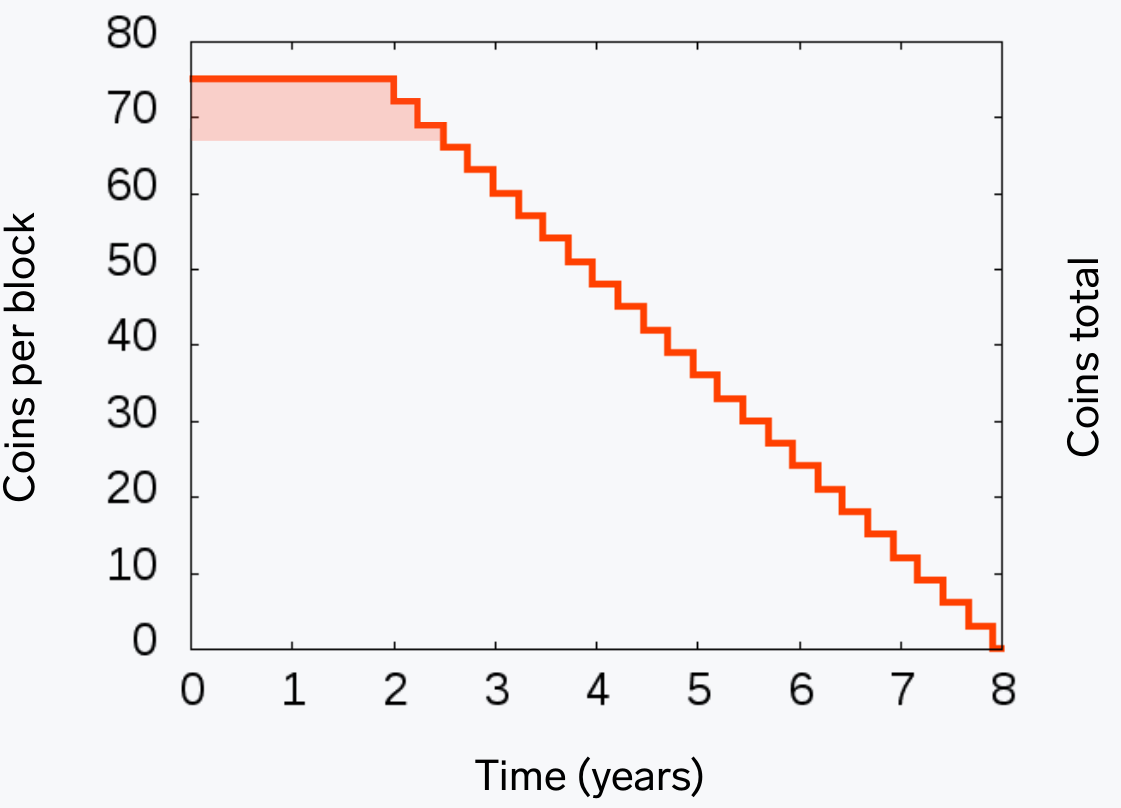
\includegraphics[width=\textwidth]{emission.png}
        \caption{Ergo emission curve
        \label{fig:emission} }
    \end{figure}


    \section{Applicability}

    To survive, a blockchain must have a user base.
    DApps and offchain protocols may be implemented in a really decentralized way due to light clients,
    however they also require useful and safe smart contracts language.
    Ergo smart contracts are based on Bitcoin-like UTXO model, where every output is protected by some script.
    If scripting language is rich enough, it allows to write Turing-complete contracts~\cite{chepurnoy2018self}
    while avoiding ad-hoc solutions for program halting like gas in Ethereum.
    Ergo script only contains operations, that allow to estimate script complexity before execution,
    preventing various DoS attacks.
    However this instructions set is enough to easily write any possible program.
    Cryptographic part of Ergo script is based on sigma protocols and naturally supports
    threshold m-of-n signatures, ring signatures and more.


    \section{Conclusions}

    \dnote{looks like no space for it, but may be useful}


    \bibliography{references}

\end{document}